\documentclass[10pt, a4paper]{article}

\usepackage[utf8]{inputenc}
\usepackage[english,spanish]{babel}
\usepackage[left=25mm, right=25mm, top=35mm, bottom=30mm, headheight=35mm]{geometry}
\usepackage{graphicx}
\usepackage{xcolor}
\usepackage{fancyhdr}
\usepackage{hyperref}
\usepackage{setspace}
\usepackage{float}
\usepackage{listings}
\lstset{
  basicstyle=\ttfamily,
  keywordstyle=\color{blue},
  commentstyle=\color{green},
  stringstyle=\color{red},
  showstringspaces=false,
  breaklines=true,
  frame=single,
  backgroundcolor=\color{lightgray},
  columns=fullflexible
}
\lstdefinestyle{JavaStyle}{
    language=Java,
    basicstyle=\small\ttfamily,
    keywordstyle=\color{blue},
    commentstyle=\color{green},
    stringstyle=\color{purple},
    tabsize=4,
    showspaces=false,
    showstringspaces=false
} 
\lstdefinestyle{JavaScriptStyle}{
    language=JavaScript,
    basicstyle=\small\ttfamily,
    keywordstyle=\color{blue},
    commentstyle=\color{green},
    stringstyle=\color{purple},
    tabsize=4,
    showspaces=false,
    showstringspaces=false
} 

% Define background color
\definecolor{background}{HTML}{2E3440}

% Syntax customization
\usepackage{minted}
\usemintedstyle{nord}
\setminted{bgcolor=background}
\setminted{breaklines}

% Variables
\newcommand{\university}{Universidad Nacional de San Agustín de Arequipa}
\newcommand{\faculty}{Facultad de Ingeniería de Producción y Servicios}
\newcommand{\program}{Escuela Profesional de Ingeniería de Sistemas}
\newcommand{\semester}{2024 - A}
\newcommand{\course}{img/web_programming}
\newcommand{\topic}{img/Python.png} 
\newcommand{\professor}{Carlo Jose Luis Corrales Delgado}
\newcommand{\students}{Mamani Anahua, Victor Narciso} 
\newcommand{\github}{https://github.com/VictorMA18/Lab05-Python}
\newcommand{\mydate}{7 de mayo, 2024}

% Just parts and chapters numbered
\setcounter{secnumdepth}{0}

% Head and foot customization
\pagestyle{fancy}
\lhead{\raisebox{-0.2\height}{
\includegraphics[width=4cm]{img/logo_unsa.png}}}
\chead{\fontsize{8}{8}\selectfont \university \\ \faculty \\ \textbf{\program}}
\rhead{\raisebox{-0.2\height}{
\includegraphics[width=3.5cm]{img/logo_episunsa.png}}}
% \lfoot{Estudiante \student}
\lfoot{Semestre \semester}
\cfoot{}
\rfoot{Pág. \thepage}

\begin{document}

\begin{titlepage}
	\centering
	\includegraphics[width=14cm]{\course} \par
  \vfill \vfill
	\includegraphics[width=15cm]{\topic}\par
  \vfill \vfill
  {\textbf{Profesor(a):} \par}
	\professor \vfill
  {\textbf{Estudiantes:} \par}
	\students \vfill
  {\textbf{Repositorio GitHub:} \par}
  \href{\github}{\github} \vfill
	{\large \mydate \par}
\end{titlepage}

\section{Ejercicios de Python}
Para iniciar los ejercicios vamos a primero instalar un paquete de python el cual es 
\begin{lstlisting}[language=bash]
  pip install pygame
\end{lstlisting} 

\section{Primer Ejercicio}
Para esto vamos poner el primer codigo python el cual es:  
\begin{figure}[H]
  \centering
  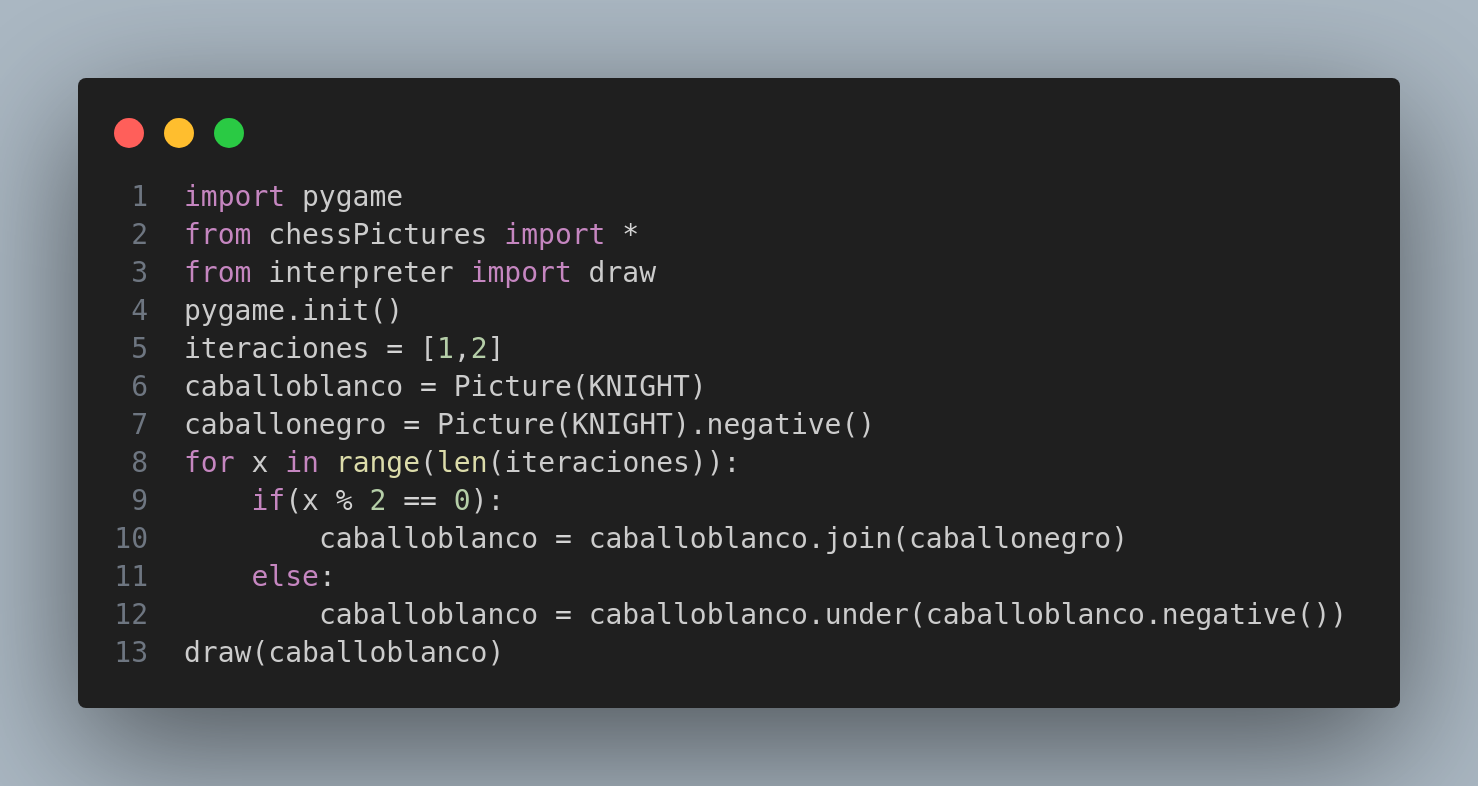
\includegraphics[width=0.7\textwidth]{img/Ej1.png}
  \caption{Ejecucion}
\end{figure}

\section{Segundo Ejercicio}
Para esto vamos poner el segundo codigo python el cual es:  
\begin{figure}[H]
  \centering
  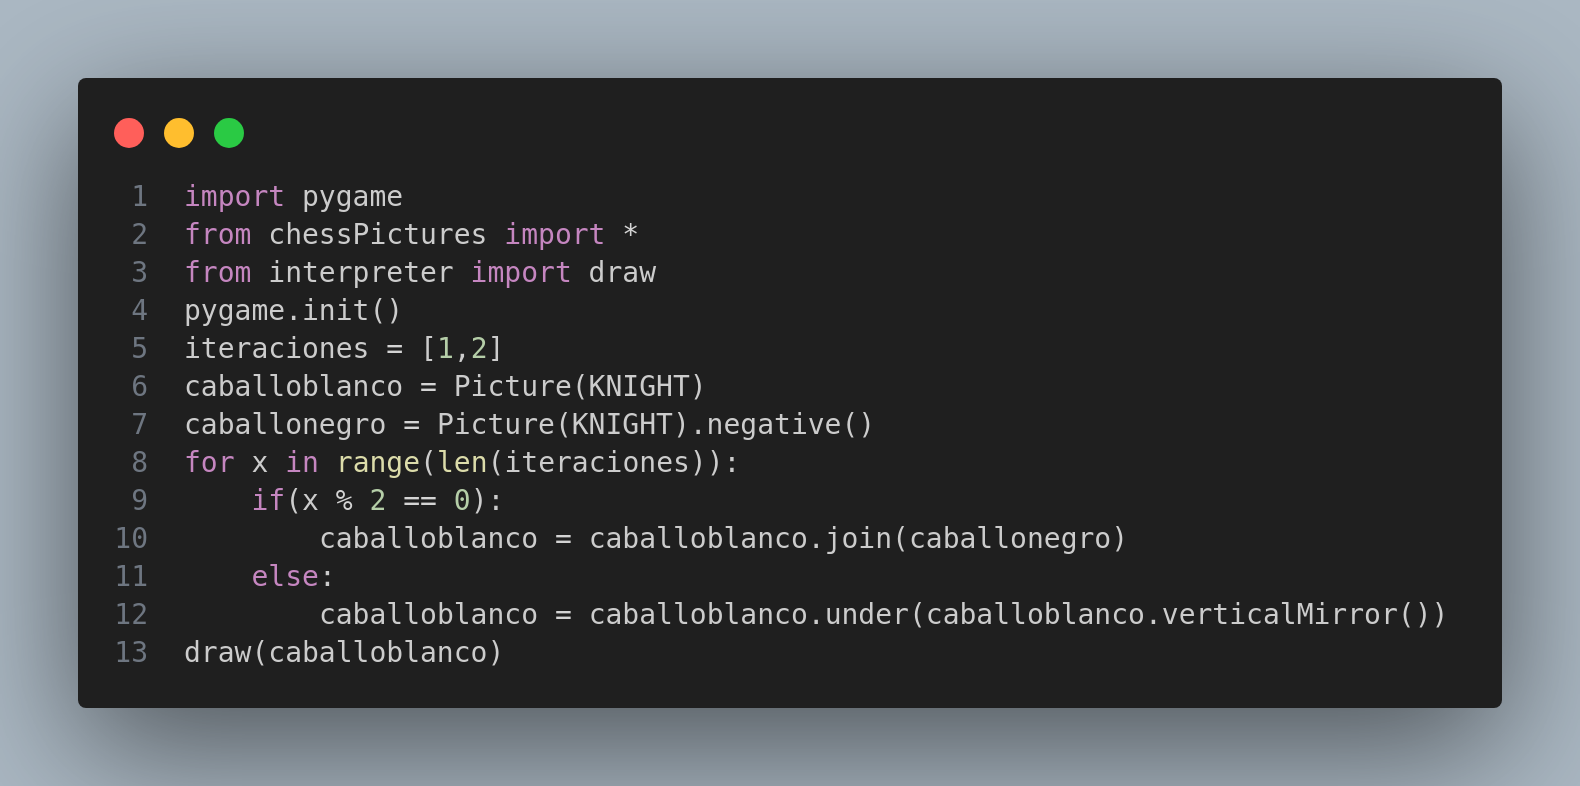
\includegraphics[width=0.7\textwidth]{img/Ej2.png}
  \caption{Ejecucion}
\end{figure}

\section{Tercer Ejercicio}
Para esto vamos poner el tercer codigo python el cual es:  
\begin{figure}[H]
  \centering
  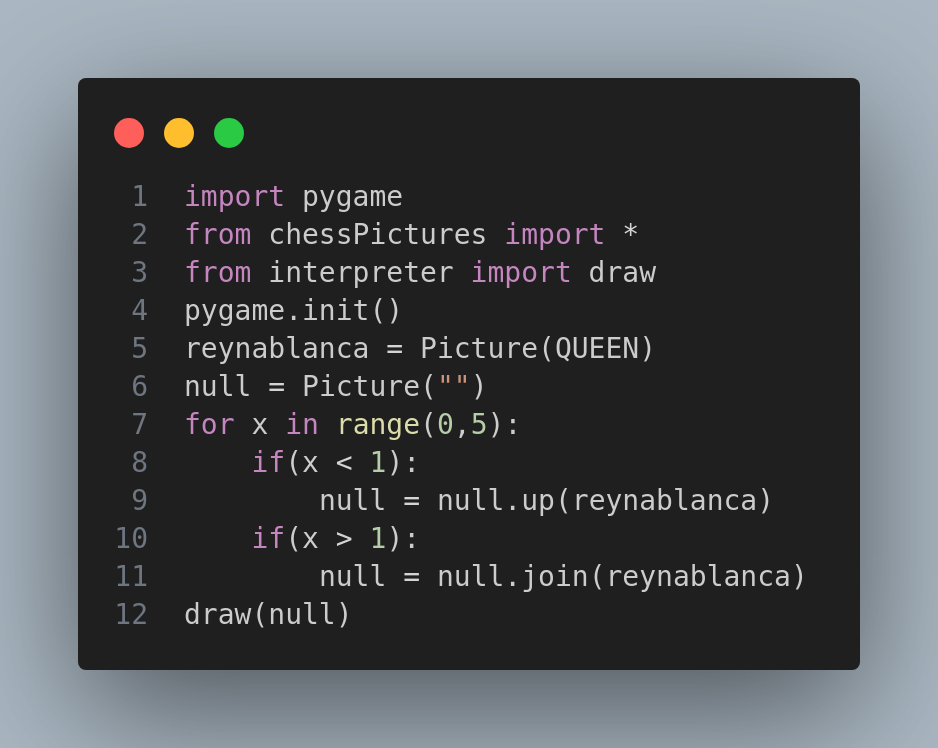
\includegraphics[width=0.7\textwidth]{img/Ej3.png}
  \caption{Ejecucion}
\end{figure}

\end{figure}
\item \textbf{URL de video de explicación:} \url{https://drive.google.com/file/d/1FKJIwx4yqkJdi3IXroJYgPwxZLg_5Hz0/view?usp=sharing}
\item \textbf{URL de repositorio de GitHub:} \url{https://github.com/VictorMA18/Lab03-Javascript}
\end{document}


